\documentclass[aspectratio=1610]{beamer}
\usepackage[utf8]{inputenc}
\usepackage{polski}
\usepackage[T1]{fontenc}
\usepackage{tikz}
\usepackage{tikzducks}
% \usetikzlibrary{decorations.pathmorphing}
\usepackage{multimedia}
\usepackage{graphicx}
\usepackage[
  % justification=centering, 
  font=scriptsize,
  figurename=rysunek
]{caption}
\captionsetup{singlelinecheck=off}
\captionsetup[figure]{textfont={small}}
\setbeamerfont{caption}{size=\small}
\usepackage{textcomp}
\usepackage{appendixnumberbeamer}
\usepackage{qrcode}
% \usepackage[natbib, language=polish, sorting=none]{biblatex}
% \addbibresource{lio.bib}
\usepackage{hyperref}
%\usepackage[width=\textwidth]{animate}
%\usepackage{chemformula}
\usepackage{sidecap}
\usepackage{multirow}
\usepackage{multicol}
\usepackage{rotating}
\usepackage{anyfontsize} % change font size for semposiwko

% \usepackage{physics}
\usepackage{array}
\usepackage{booktabs}
\usepackage{transparent}
\usepackage{siunitx}
% \usepackage[rightcaption]{sidecap}
\usepackage{eso-pic}

\usepackage{amsmath,amsthm,amssymb}
\DeclareMathOperator{\sgn}{sgn}

\usepackage{listings}
\lstset{
basicstyle=\small\ttfamily,
columns=flexible,
breaklines=true
}

% \usepackage{emoji}
\usepackage{subcaption}
% \usepackage{enumerate}

\usepackage[natbib, sorting=none, style=authoryear]{biblatex}
% \usepackage{bibentry}
\addbibresource{lio.bib}
\renewcommand*{\bibfont}{\scriptsize}

\usefonttheme[onlymath]{serif}

\usetheme{Szeged}
\usecolortheme{whale}
\setbeamercolor{palette primary}{bg=violet!80!black,fg=white}
\setbeamercolor{palette secondary}{bg=violet!60!black,fg=white}
% \definecolor{deepviolet}{RGB}{46,0,79}
% \definecolor{vividpink}{RGB}{255,0,127}
% \setbeamercolor{palette primary}{bg=deepviolet,fg=white}
% \setbeamercolor{palette secondary}{bg=vividpink,fg=white}
\setbeamercolor{palette tertiary}{bg=violet!40!black,fg=white}
\setbeamercolor{palette quaternary}{bg=violet!20!black,fg=white}
\setbeamercolor{structure}{fg=violet!60!black}
% \setbeamertemplate{caption}{\insertcaption}
% \setbeamertemplate{headline}{
%   \begin{beamercolorbox}[wd=.9\paperwidth]{headline}
%     \vspace{1.5ex}
%     \insertsectionnavigationhorizontal
%     \vspace{1.5ex}
%   \end{beamercolorbox}
% }
% \definecolor{violet-dark}{HTML}{4B0082}
% \definecolor{teal}{HTML}{008080}
% \definecolor{amber}{HTML}{FFC107}
% \definecolor{light-grey}{HTML}{F5F5F5}
% \definecolor{charcoal}{HTML}{333333}
% \setbeamercolor{palette primary}{bg=violet-dark, fg=white}
% \setbeamercolor{palette secondary}{bg=teal, fg=white}
% \setbeamercolor{palette tertiary}{bg=amber, fg=charcoal}
% \setbeamercolor{background canvas}{bg=light-grey}
% \setbeamercolor{normal text}{fg=charcoal}
% Główna paleta fioletów
% \definecolor{coolblack}{HTML}{000000}
% \definecolor{coolnavy}{HTML}{14213D}
% \definecolor{coolorange}{HTML}{FCA311}
% \definecolor{coollightgray}{HTML}{E5E5E5}
% \definecolor{coolwhite}{HTML}{FFFFFF}

% % Opcjonalnie: ustawienia kolorów dla Beamera
% \setbeamercolor{normal text}{fg=coolblack,bg=coolwhite}
% \setbeamercolor{structure}{fg=coolorange}
% \setbeamercolor{frametitle}{fg=coolwhite,bg=coolnavy}
% \setbeamercolor{title}{fg=coolwhite,bg=coolnavy}
% \setbeamercolor{item}{fg=coolorange}
% \setbeamercolor{block title}{fg=coolwhite,bg=coolnavy}
% \setbeamercolor{block body}{fg=coolblack,bg=coollightgray}
% \setbeamercolor{palette tertiary}{fg=coolwhite, bg=coolorange}
% \setbeamercolor{palette quaternary}{fg=coolblack, bg=coollightgray}

\linespread{0.8}

\setbeamertemplate{background}%
{%
    \begin{tikzpicture}[remember picture,overlay]{\node[yshift=1.5cm,xshift=-2cm,opacity=0.1] at (current page.south east)
      {
      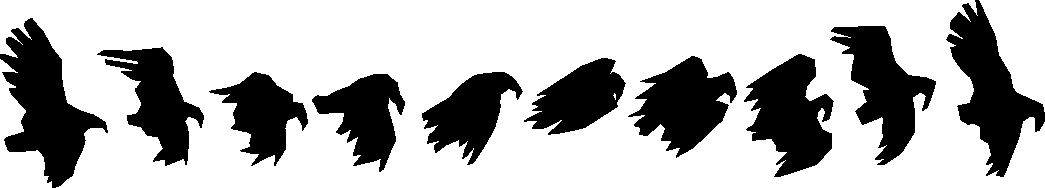
\includegraphics[scale=0.4, angle=25]{ptaki.pdf}
      }
      ;
    \node[yshift=-2cm,xshift=-2cm,opacity=0.1] at (current page.north east)
      {
      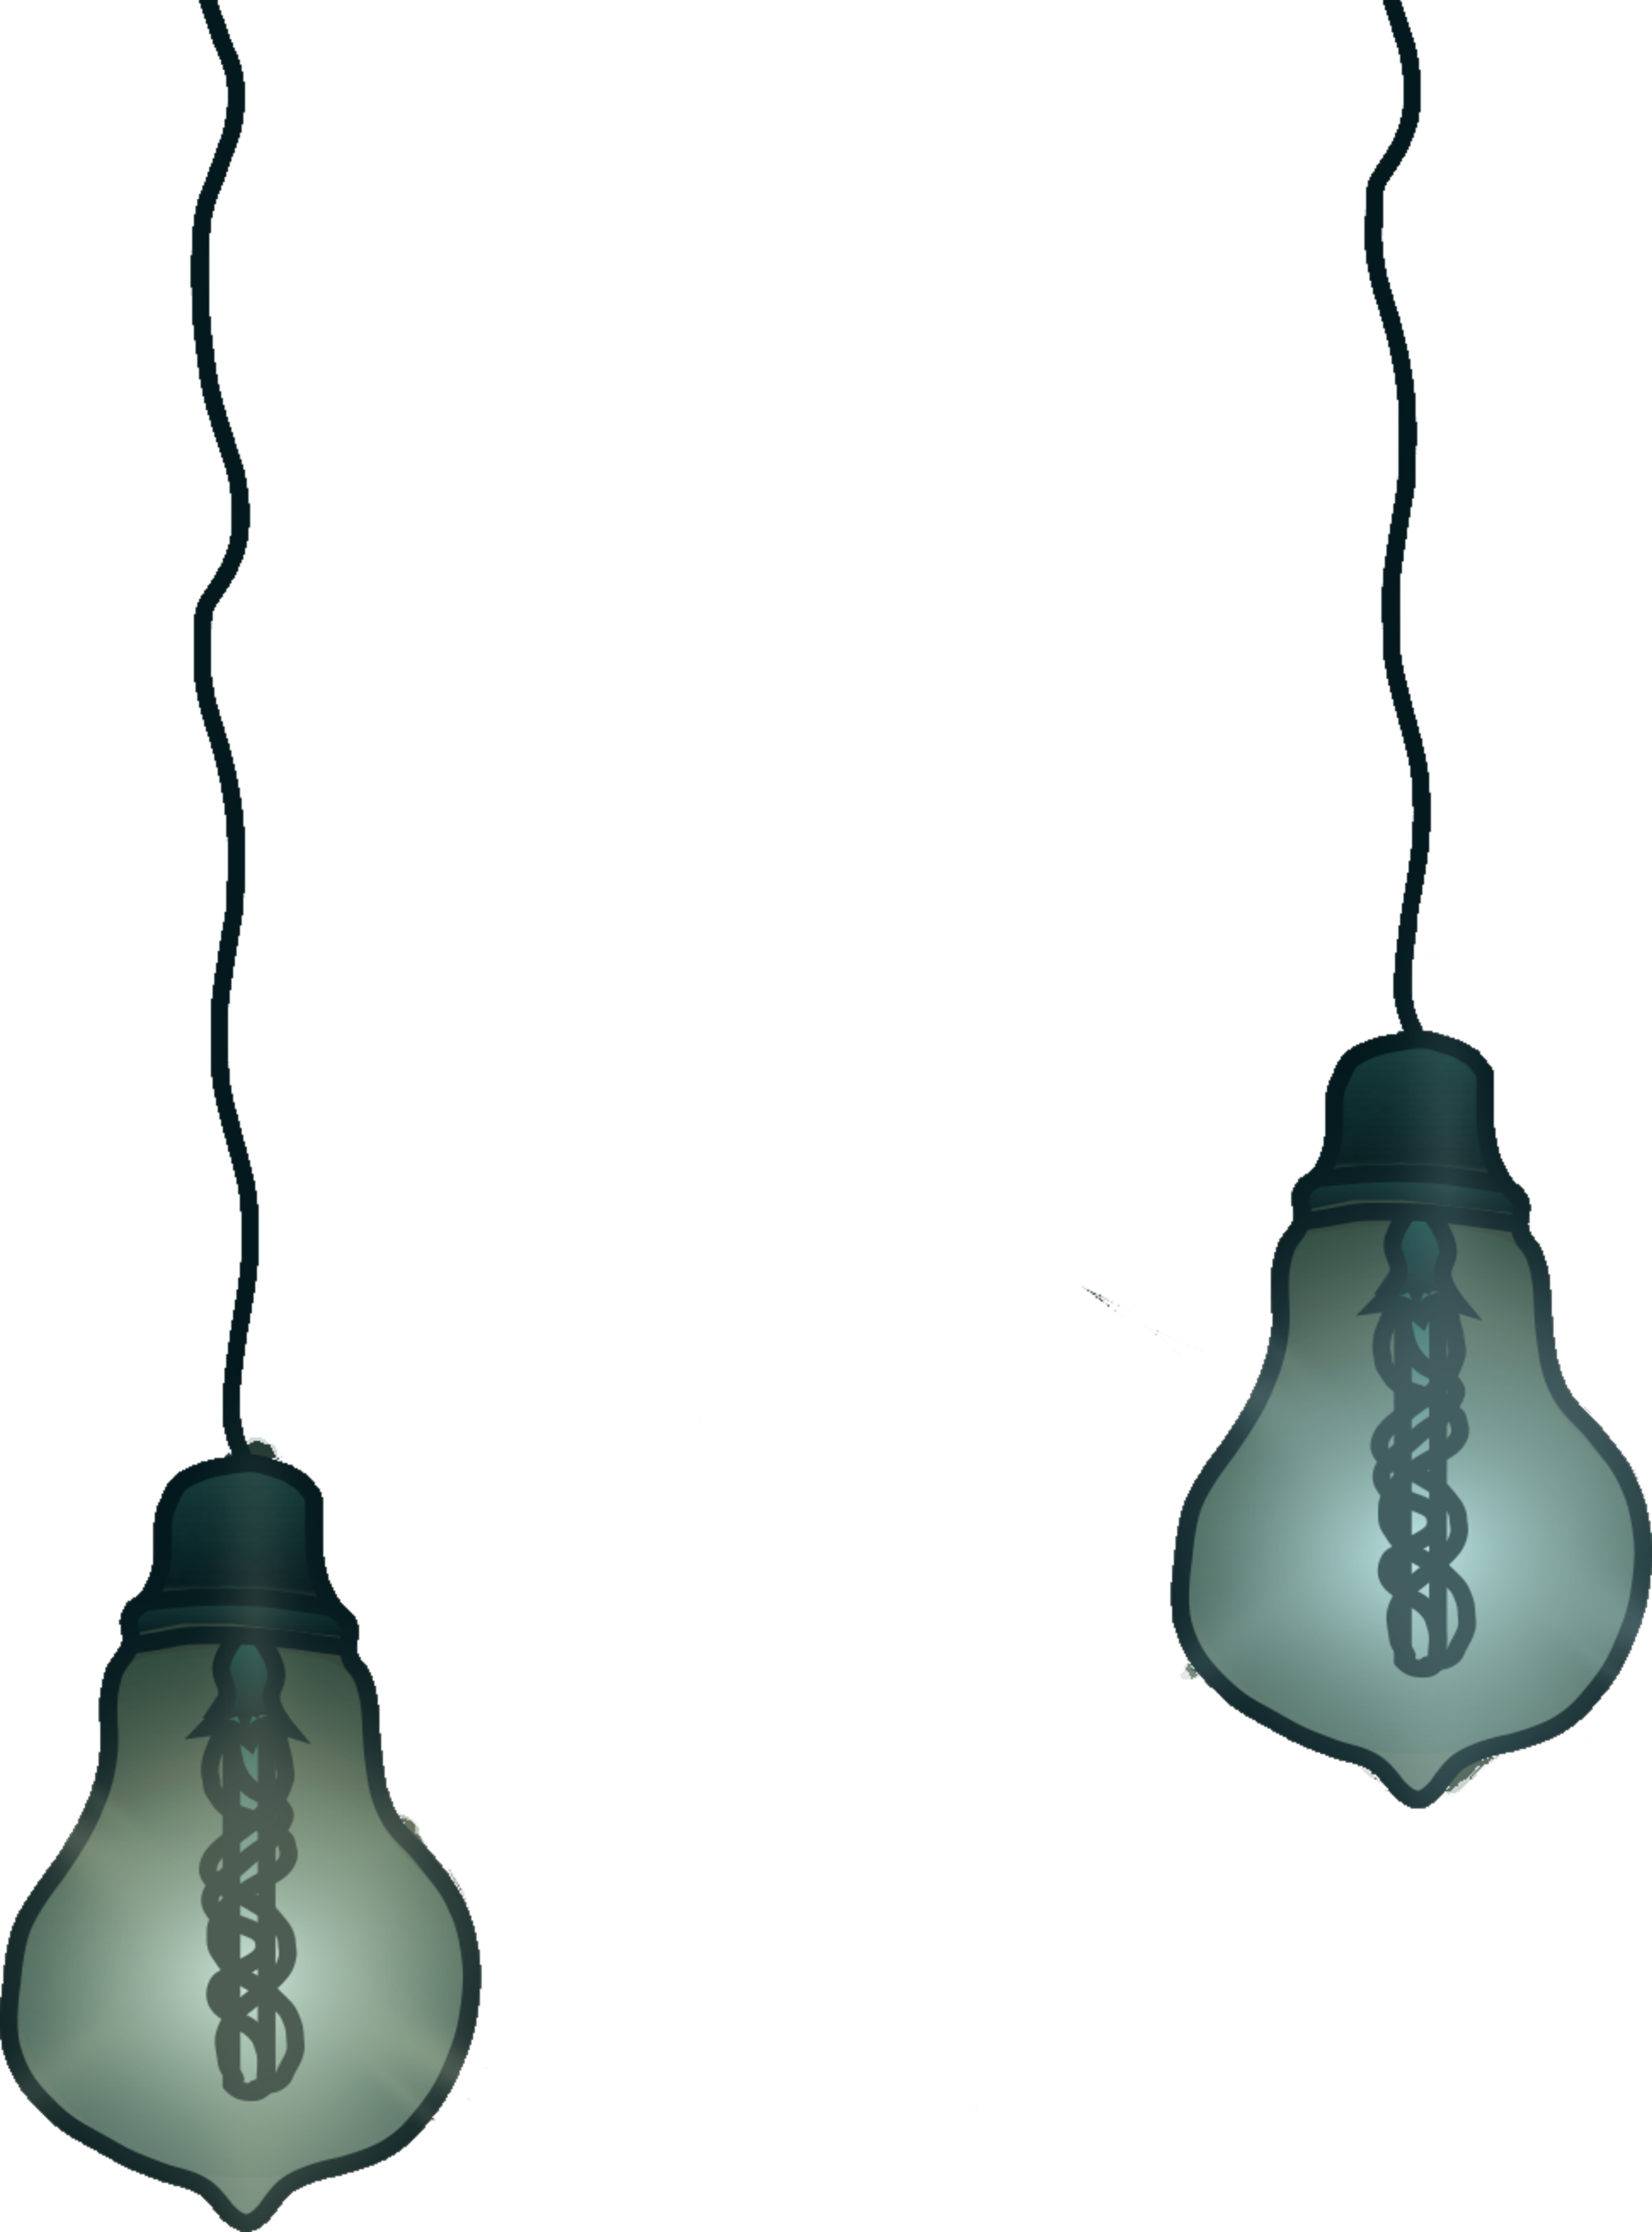
\includegraphics[scale=0.1, angle=0]{zarowki.pdf}
      }
      ;
    \node[yshift=1.0cm,xshift=0.6cm] (logopos) at (current page.south west) {{\begin{tikzpicture}\shuffleducks\duck[signpost=\insertframenumber, \randomhead,scale=.4]\end{tikzpicture}}};
    \pgfmathsetmacro{\progress}{360*(\insertframenumber)/(\inserttotalframenumber)}%;
    \draw[line width=0.2*3pt] ([xshift=0.55cm] logopos)  arc[radius=0.55cm, start angle=0, end angle=\progress];
    \fill ([shift={(\progress:0.55cm)}] logopos) circle(1pt);

    }
        \end{tikzpicture}
    
}

\newcommand{\SeMPowisko}{%
\large S\normalsize%
\kern-.3em \lower.2ex\hbox{e}%
\lower.2ex\hbox{\large M\normalsize}%
\kern-.1em \raise.1ex\hbox{\large P\normalsize}%
\kern-.3em \lower.2ex\hbox{o}%
\kern-.2em \raise.2ex\hbox{w}%
\lower.2ex\hbox{i}%
s%
\raise.2ex\hbox{k}%
\kern-.3em \lower.2ex\hbox{o}%
}
% \usepackage{microtype}
% \DeclareRobustCommand{\SeMPowisko}{SeMPowisko}


% \newcommand\Tikz{Ti\emph{k}Z}
% \definecolor{neworange}{RGB}{255,140,0}
% \renewcommand{\figurename}{figure}

\setbeamersize{text margin left=1.3cm, text margin right=1.3cm}


\title{jak zobaczyć siły komórkowe?}
\subtitle{mądry podtytuł}
\author[M. Winiarski]{Mateusz ,,\(\blacksquare\)'' Winiarski
% \\{\scriptsize i pomocnicy z obozów reedukacyjnych w Sinciangu}
}
\institute[fais uj]{(bio)fizyka\(^\dagger\), FAIS, Uniwersytet Jagielloński} 
\date[dzisiaj]{dzisiaj, \today}

\newcommand{\um}{\si{\micro\meter}}

\begin{document}

\nocite{Trepat_2020,
Harris_Wild_Stopak_1980,
Weiss_1934,
Dembo_Wang_1999,
Butler_Tolić-Nørrelykke_Fabry_Fredberg_2002}
\frame{\titlepage}

\begin{frame}{problem}{}
  % \the\textwidth
  \begin{figure}
 \centering
 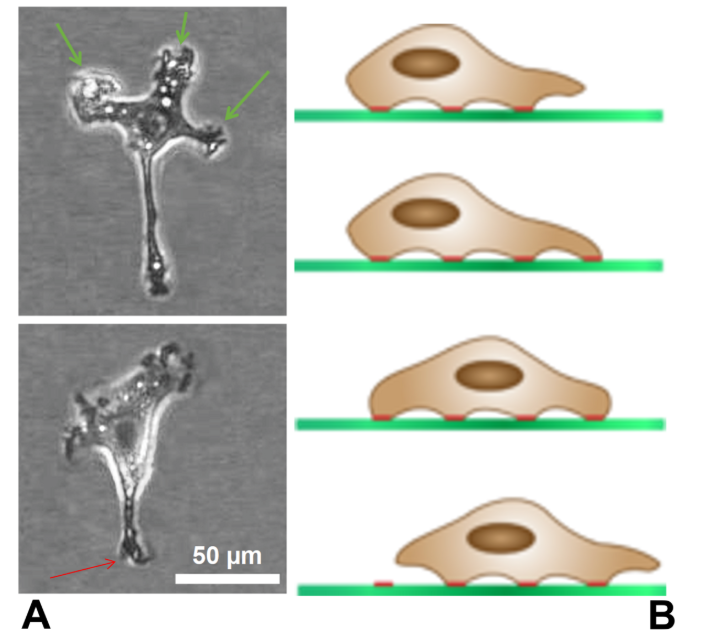
\includegraphics[width=0.5\textwidth]{images/2025-12-19-13-11-38.png}
 \caption{ruchliwa komórka, np. komórka nerwowa albo tkanki łącznej (źródło: wikipedia)}
 \end{figure}
\end{frame}

\begin{frame}{rozwiązanie I: guma silikonowa}{}
\begin{itemize}
  \item artykuł: \cite{Harris_Wild_Stopak_1980}
  \item podłoże: polidimetylosiloksan (PDMS)
  \item przygotowanie: usieciowanie (palnikiem) warstwy o grubości 1 \si{\micro\meter}
\end{itemize}
\end{frame}


\begin{frame}{problem}{}
 
\begin{figure}
 \centering
 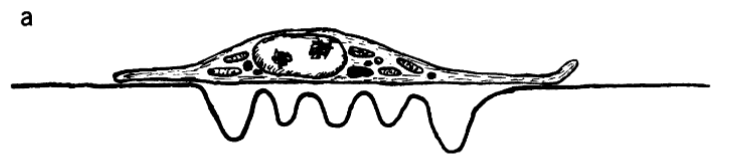
\includegraphics[width= 0.94023  \textwidth]{images/2025-12-17-11-33-57.png}
 \caption{komórka (fibroblast) pełznie po podłożu (źródło: \cite{Harris_Wild_Stopak_1980})}
 \end{figure}

\end{frame}

\begin{frame}{problem}{}

\begin{figure}
 \centering
 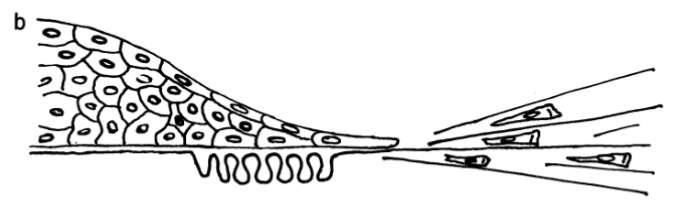
\includegraphics[width=0.94023 \textwidth]{images/2025-12-17-11-41-12.png}
 \caption{widok z boku brzegu skupiska komórek (eksplantat) (źródło: \cite{Harris_Wild_Stopak_1980})}
 \end{figure}
  
\end{frame}


\begin{frame}{rozwiązanie I: guma silikonowa}{}
  \begin{figure}
 \centering
 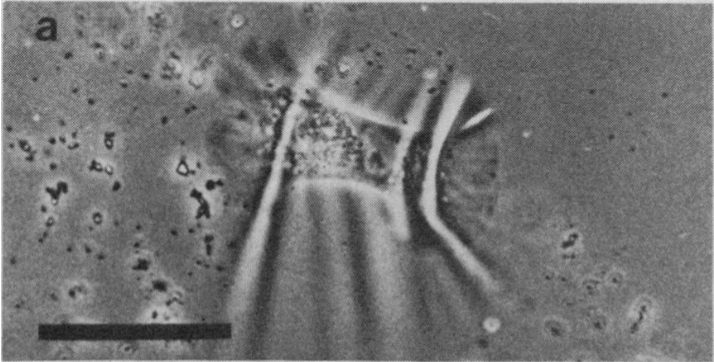
\includegraphics[width=0.83576 \textwidth]{images/2025-12-17-12-22-40.png}
 \caption{pojedynczy fibroblast serca kury. widać komórkę oraz zmarszczki w podłożu silikonowym stworzone podczas ruchu (źródło: \cite{Harris_Wild_Stopak_1980}) (skala 50 \um)}
 \end{figure}
\end{frame}

\begin{frame}{guma}{}
  \begin{figure}
 \centering
 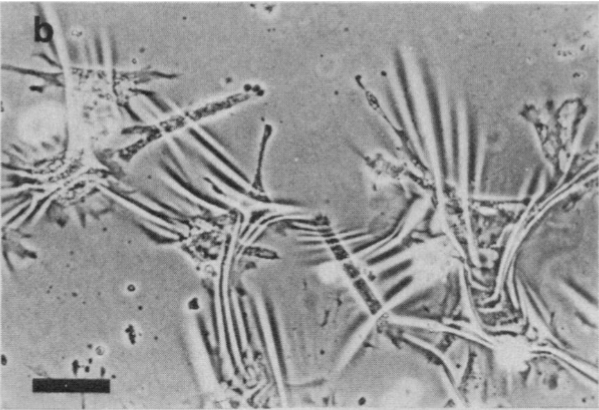
\includegraphics[width=0.679055\textwidth]{images/2025-12-17-12-59-19.png}
 \caption{kilkanaście fibroblastów. wzór deformacji jest wypadkową deformacji od wielu niezależnie poruszających się komórek (źródło: \cite{Harris_Wild_Stopak_1980}) (skala 100 \um)}
 \end{figure}
\end{frame}

% \begin{frame}{puma}{}
%   \begin{figure}
%  \centering
%  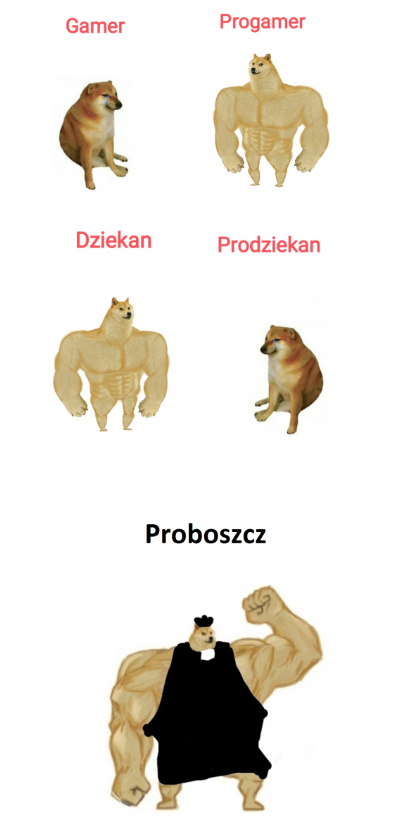
\includegraphics[width=0.52235 \textwidth]{images/2025-12-17-13-16-18.png}
%  \caption{}
%  \end{figure}
% \end{frame}

\begin{frame}{guma}{}

  \begin{figure}
 \centering
 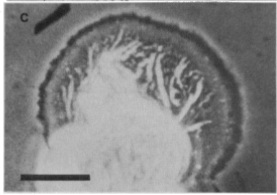
\includegraphics[width=0.7\textwidth]{images/2025-12-19-12-19-57.png}
 \caption{klatka z filmu pokazująca poczatek ruchu komórki linii PTK-1. ciemna obwódka pokazuje gdzie warstwa jest rozciągana (źródło: \cite{Harris_Wild_Stopak_1980}) (skala 20 \um)}
 \end{figure}
  
\end{frame}

\begin{frame}{puma}{}
  \begin{figure}
 \centering
 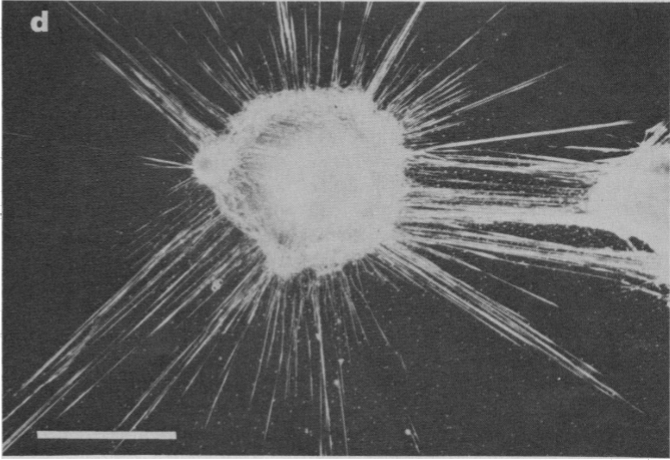
\includegraphics[width=0.62682 \textwidth]{images/2025-12-17-13-25-19.png}
 \caption{zdjęcie fibroblastów w technice ciemnego pola\footnote{oświetlanie pod dużym kątem i obserwacja światła rozproszonego} po 48h. widoczne dwa centra w~miejscach dwóch eksplanatów (źródło: \cite{Harris_Wild_Stopak_1980}) (skala 1 mm)}
 \end{figure}
\end{frame}

\begin{frame}{cofamy się do 1934}{}
  \begin{figure}
 \centering
 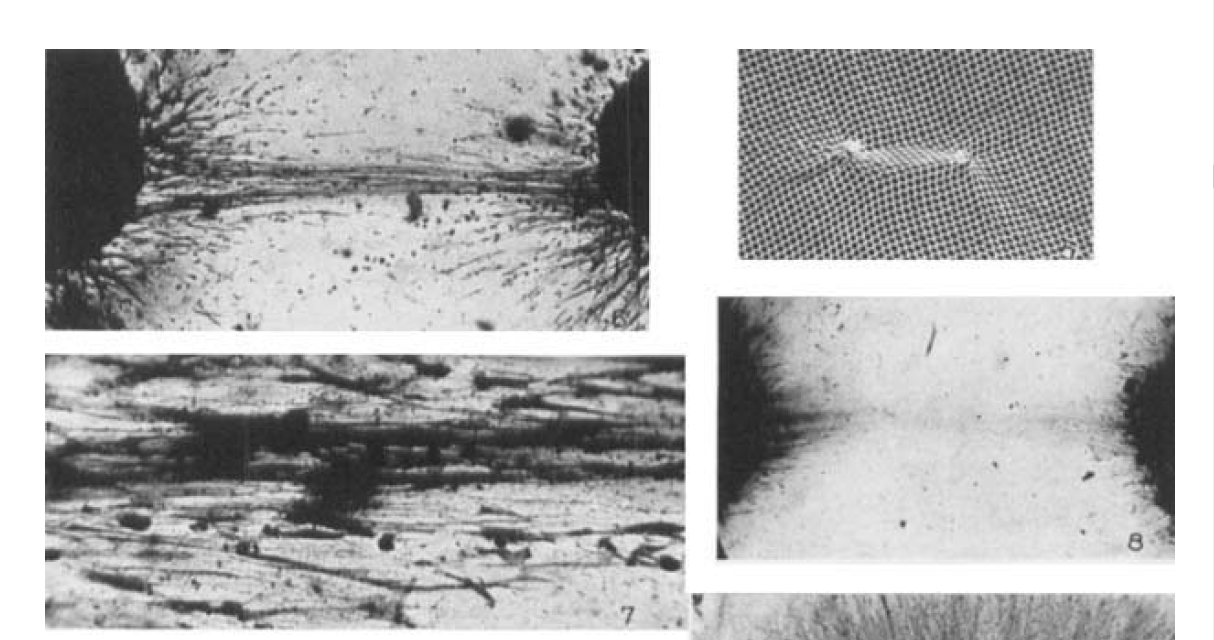
\includegraphics[width=0.8 \textwidth]{images/2025-12-18-11-50-25.png}
 \caption{(a) model pokazujący orientację naprężeń w systemie oraz (b,c,d) rzeczywiste struktury komórek i włókien nerwowych na osoczu krwi (źródło: \cite{Weiss_1934})}
 \end{figure}
\end{frame}

\begin{frame}{rozwiązanie II: poliakrylamid (1999)}{}
\begin{itemize}
  \item artykuł: \cite{Dembo_Wang_1999}
  \item podłoże: żel poliakrylamidowy
  \item przygotowanie: umieszczenie kulek fluorescencyjnych i pokrycie kolagenem
\end{itemize}
\end{frame}

% \begin{frame}{metodologia}{}
% \begin{figure}
%   \begin{subfigure}{0.48\textwidth}
%  \centering
%  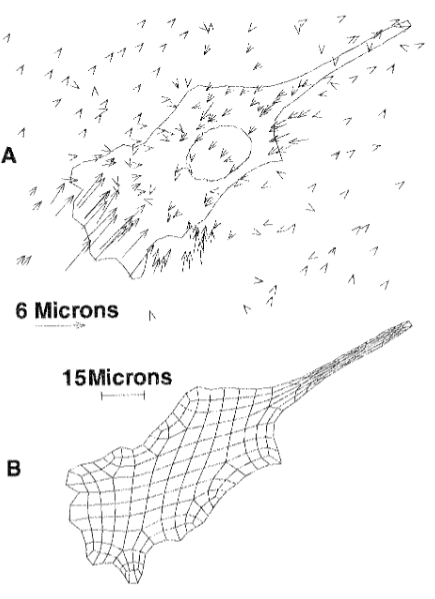
\includegraphics[width=0.7\textwidth]{images/2025-12-19-13-22-00.png}
% %  \caption{}
%  \end{subfigure}
%  \begin{subfigure}{0.48\textwidth}
%  \centering
%  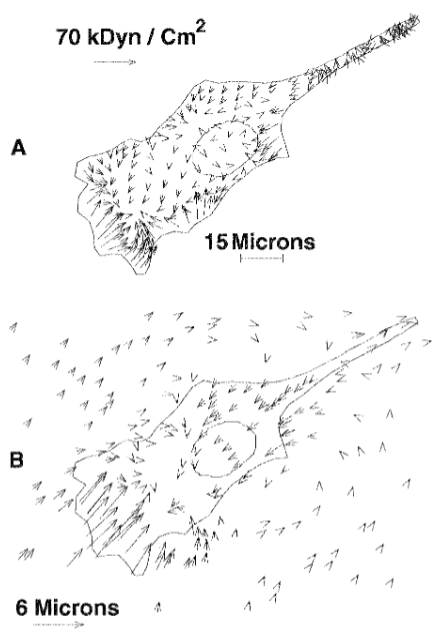
\includegraphics[width=0.7\textwidth]{images/2025-12-19-13-22-57.png}
% %  \caption{}
%  \end{subfigure}
% \caption{podpis pod rysunkiem}
% \end{figure}
  
% \end{frame}

\begin{frame}{metodologia I}{}

\begin{figure}
 \centering
 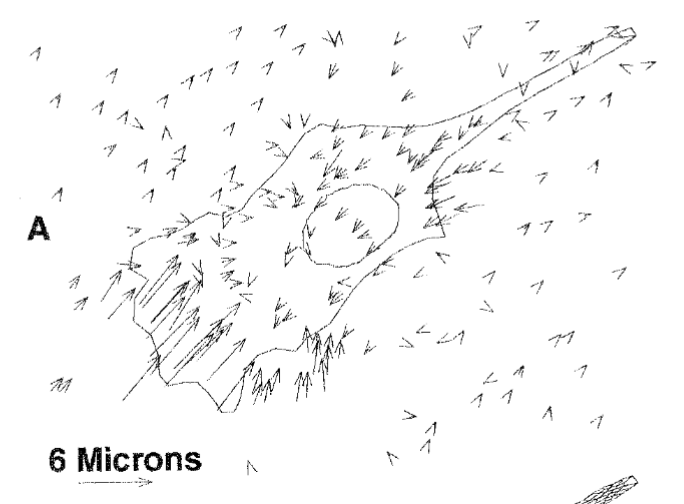
\includegraphics[width=0.7\textwidth]{images/2025-12-19-13-38-35.png}
 \caption{zmierzone przemieszczenie kulek}
 \end{figure}
  
\end{frame}

\begin{frame}{metodologia II}{}

\begin{figure}
 \centering
 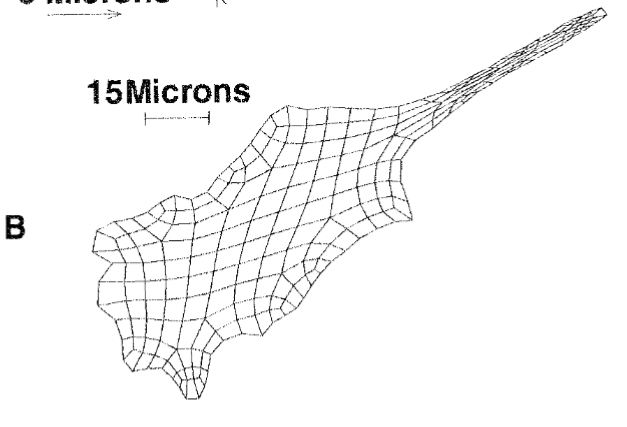
\includegraphics[width=0.7\textwidth]{images/2025-12-19-13-39-19.png}
 \caption{konstrukcja siatki obliczeniowej}
 \end{figure}
  
\end{frame}
\begin{frame}{metodologia III}{}

\begin{figure}
 \centering
 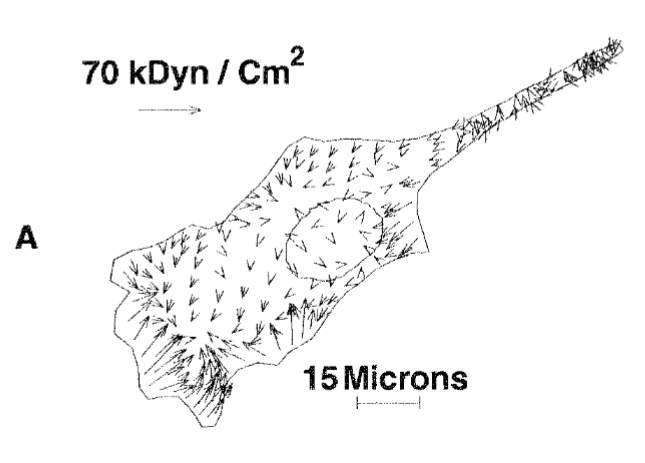
\includegraphics[width=0.7\textwidth]{images/2025-12-19-13-39-41.png}
 \caption{mapa sił trakcyjnych}
 \end{figure}
  
\end{frame}

\begin{frame}{metodologia IV}{}

\begin{figure}
 \centering
 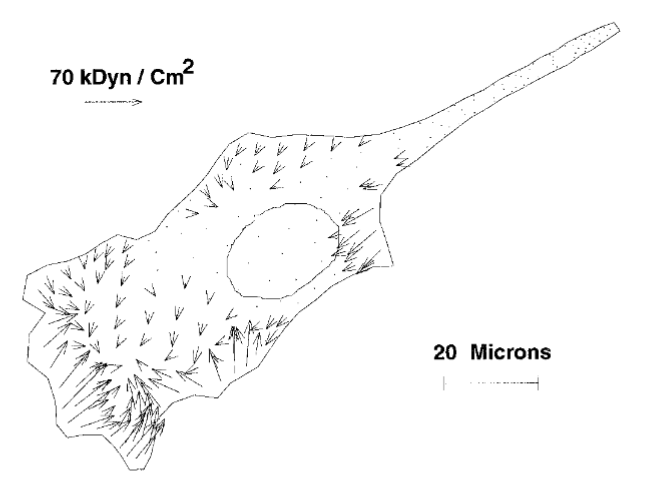
\includegraphics[width=0.7\textwidth]{images/2025-12-19-14-08-33.png}
 \caption{mapa sił trakcyjnych po przefiltrowaniu}
 \end{figure}

\end{frame}

\begin{frame}{wyniki (1999)}{}
%   \begin{figure}
%  \centering
%  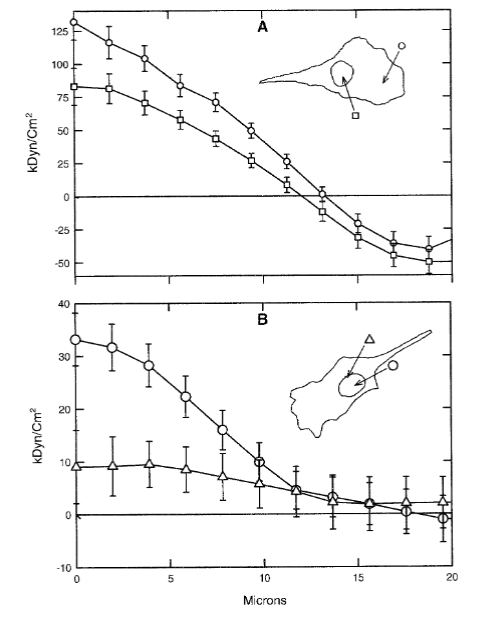
\includegraphics[width=0.5\textwidth]{images/2025-12-19-00-45-27.png}
%  \caption{(źródło: \cite{Dembo_Wang_1999})}
%  \end{figure}
\begin{figure}
\begin{subfigure}{0.45\textwidth}
 \centering
 ~
 \vspace{0.5cm}
 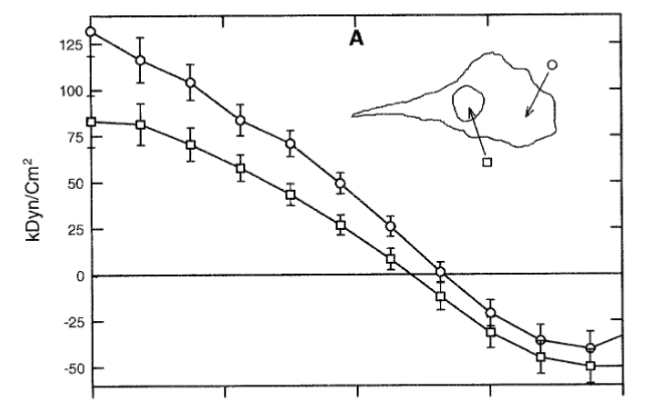
\includegraphics[width=0.95\textwidth]{images/2025-12-19-00-48-20.png}
%  \caption{}
 \end{subfigure}
 \begin{subfigure}{0.45\textwidth}
 \centering
 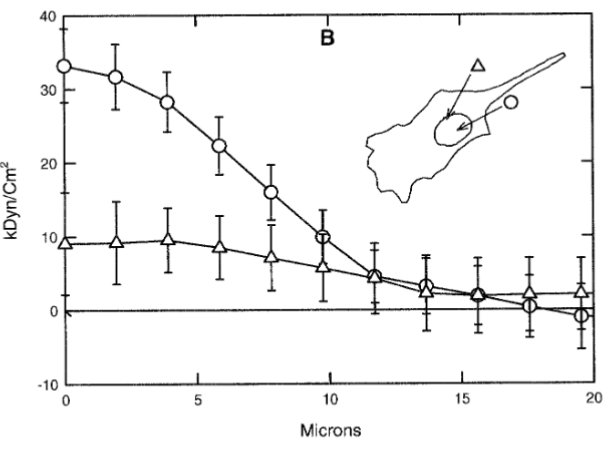
\includegraphics[width=0.95\textwidth]{images/2025-12-19-00-48-37.png}
%  \caption{}
 \end{subfigure}
 \caption{ilościowy rozkład sił trakcyjnych (ściągających) wewnątrz komórki, od strony \emph{leading edge} (A) i \emph{trailing edge} (B)(źródło: \cite{Dembo_Wang_1999})}
 \end{figure}
\end{frame}

\begin{frame}{wnioski}{}
  \begin{itemize}[<+->]
    \item podłoże jest deformowane przez siły trakcyjne
    \item siły są mierzalne
    \item \(\to\) TFM (\emph{traction force microscopy})
    \item lamellipodium ciągnie, ogon się wlecze
  \end{itemize}
\end{frame}

\begin{frame}{bibliografia}
  % \nocite{*}
  \printbibliography[heading=none]
\end{frame}


\begin{frame}{koniec}
    \begin{figure}
 \centering
 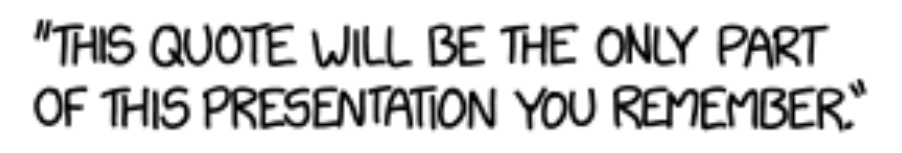
\includegraphics[width=0.6\textwidth]{images/2025-11-13-00-34-41.png}
 \end{figure}
 \begin{figure}
 \centering
 \hspace{0.25\textwidth}
\includegraphics[width=0.3\textwidth]{images/2025-11-13-00-35-06.png}
 \end{figure}
\end{frame}



\end{document}